\mysection{РАЗРАБОТКА ПРИЛОЖЕНИЯ}

\subsection{Подготовка окружения для разработки}

Основой разрабатываемого приложения является JavaScript-фреймворк Vue.js. Данный фреймворк позволяет начать работу над проектом максимально просто -- достаточно добавить на веб-страницу JavaScript-файл с~кодом Vue.js, используя тег \,\verb|<script>|.

Однако, для обеспечения удобства разработки и~возможности использования новейших возможностей языка JavaScript было решено использовать пакетный менеджер NPM \cite{NPM} вместе с~компилятором Babel \cite{Babel} и~утилитой Webpack \cite{Webpack}, предназначенной для сборки веб-приложений.


\subsubsection{Пакетный менеджер NPM}

\textbf{NPM} (аббр. \emph{Node Package Manager}) -- менеджер пакетов, входящий в~состав программной платформы Node.js \cite{NodeJS}. NPM существенно упрощает установку компонентов, необходимых для работы или сборки приложения.

При работе с~данным пакетным менеджером, особый интерес представляет файл \textbf{package.json}. Данный файл содержит информацию о~разрабатываемом приложении: название, версия, описание и~т.д (см. листинг \ref{lst:package_json}). Но наиболее важным содержимым файла package.json являются зависимости -- список имён и~версий пакетов, требующихся для работы приложения.


\subsubsection{Babel}

\textbf{Babel} -- транспилер (англ. \emph{transpiler}), транслирующий код JavaScript стандартов ES2015 и~новее \cite{ecma262} в~код более ранних версий JavaScript.

Применение данного инструмента при разработке проекта позволяет использовать возможности JavaScript, представленные в~новейших стандартах языка, не теряя при этом совместимость приложения со~старыми версиями веб-браузеров.

% TODO Пример работы Babel
% TODO Список поддерживаемых браузеров?
\lstinputlisting[
  caption={Пример содержимого файла package.json},
  label={lst:package_json}
]{src/package.json}


\subsubsection{Webpack}

\textbf{Webpack} -- система сборки для JavaScript-приложений, предназначенная, в первую очередь, для генерирования статических ресурсов на основе JavaScript-модулей и~их зависимостей.

Одним из основных преимуществ Webpack является его способность работать с~практически любыми типами ресурсов. Данная возможность обеспечивается дополнительно устанавливаемых \emph{загрузчиков} (англ. \emph{loaders}), которые, к~примеру, позволяют:
\begin{dashitemize}
  \item производить компиляцию JavaScript-файлов с~помощью Babel;
  \item осуществлять статический анализ кода с~помощью ESLint \cite{ESLint};
  \item минифицировать и обфусцировать код приложения;
  \item обрабатывать файлы с~расширением <<.vue>> (однофайловые компоненты Vue.js);
  \item производить трансляцию стилей, описанных на языке SCSS \cite{Sass}, в~CSS.
\end{dashitemize}

Стоит также отметить, что с~помощью Webpack можно существенно облегчить разработку ве-приложения. Благодаря специальным расширениям становится возможно запустить локальный HTTP-сервер, позволяющий просматривать и~отлаживать разрабатываемое приложение в~браузере компьютера, на котором ведётся разработка.



\subsection{Структура проекта. Артефакты сборки (?)}


\subsubsection{Структура проекта}

Исходный код клиентской части приложения является частью Python-проекта, написанного с использованием веб-фреймворка Flask. Подобная структура проекта позволяет держать весь код приложения в одном репозитории и облегчает сборку Python-приложения, предназначенного для установки на устройства Reach и~Reach~RS.

Код клиентского веб-приложения находится в директории \emph{static-src}. Структура данной директории подробно описана на рисунке \ref{fig:project-tree}.

\begin{figure}[h!]
  \centering
  \setlength{\fboxsep}{5pt}
  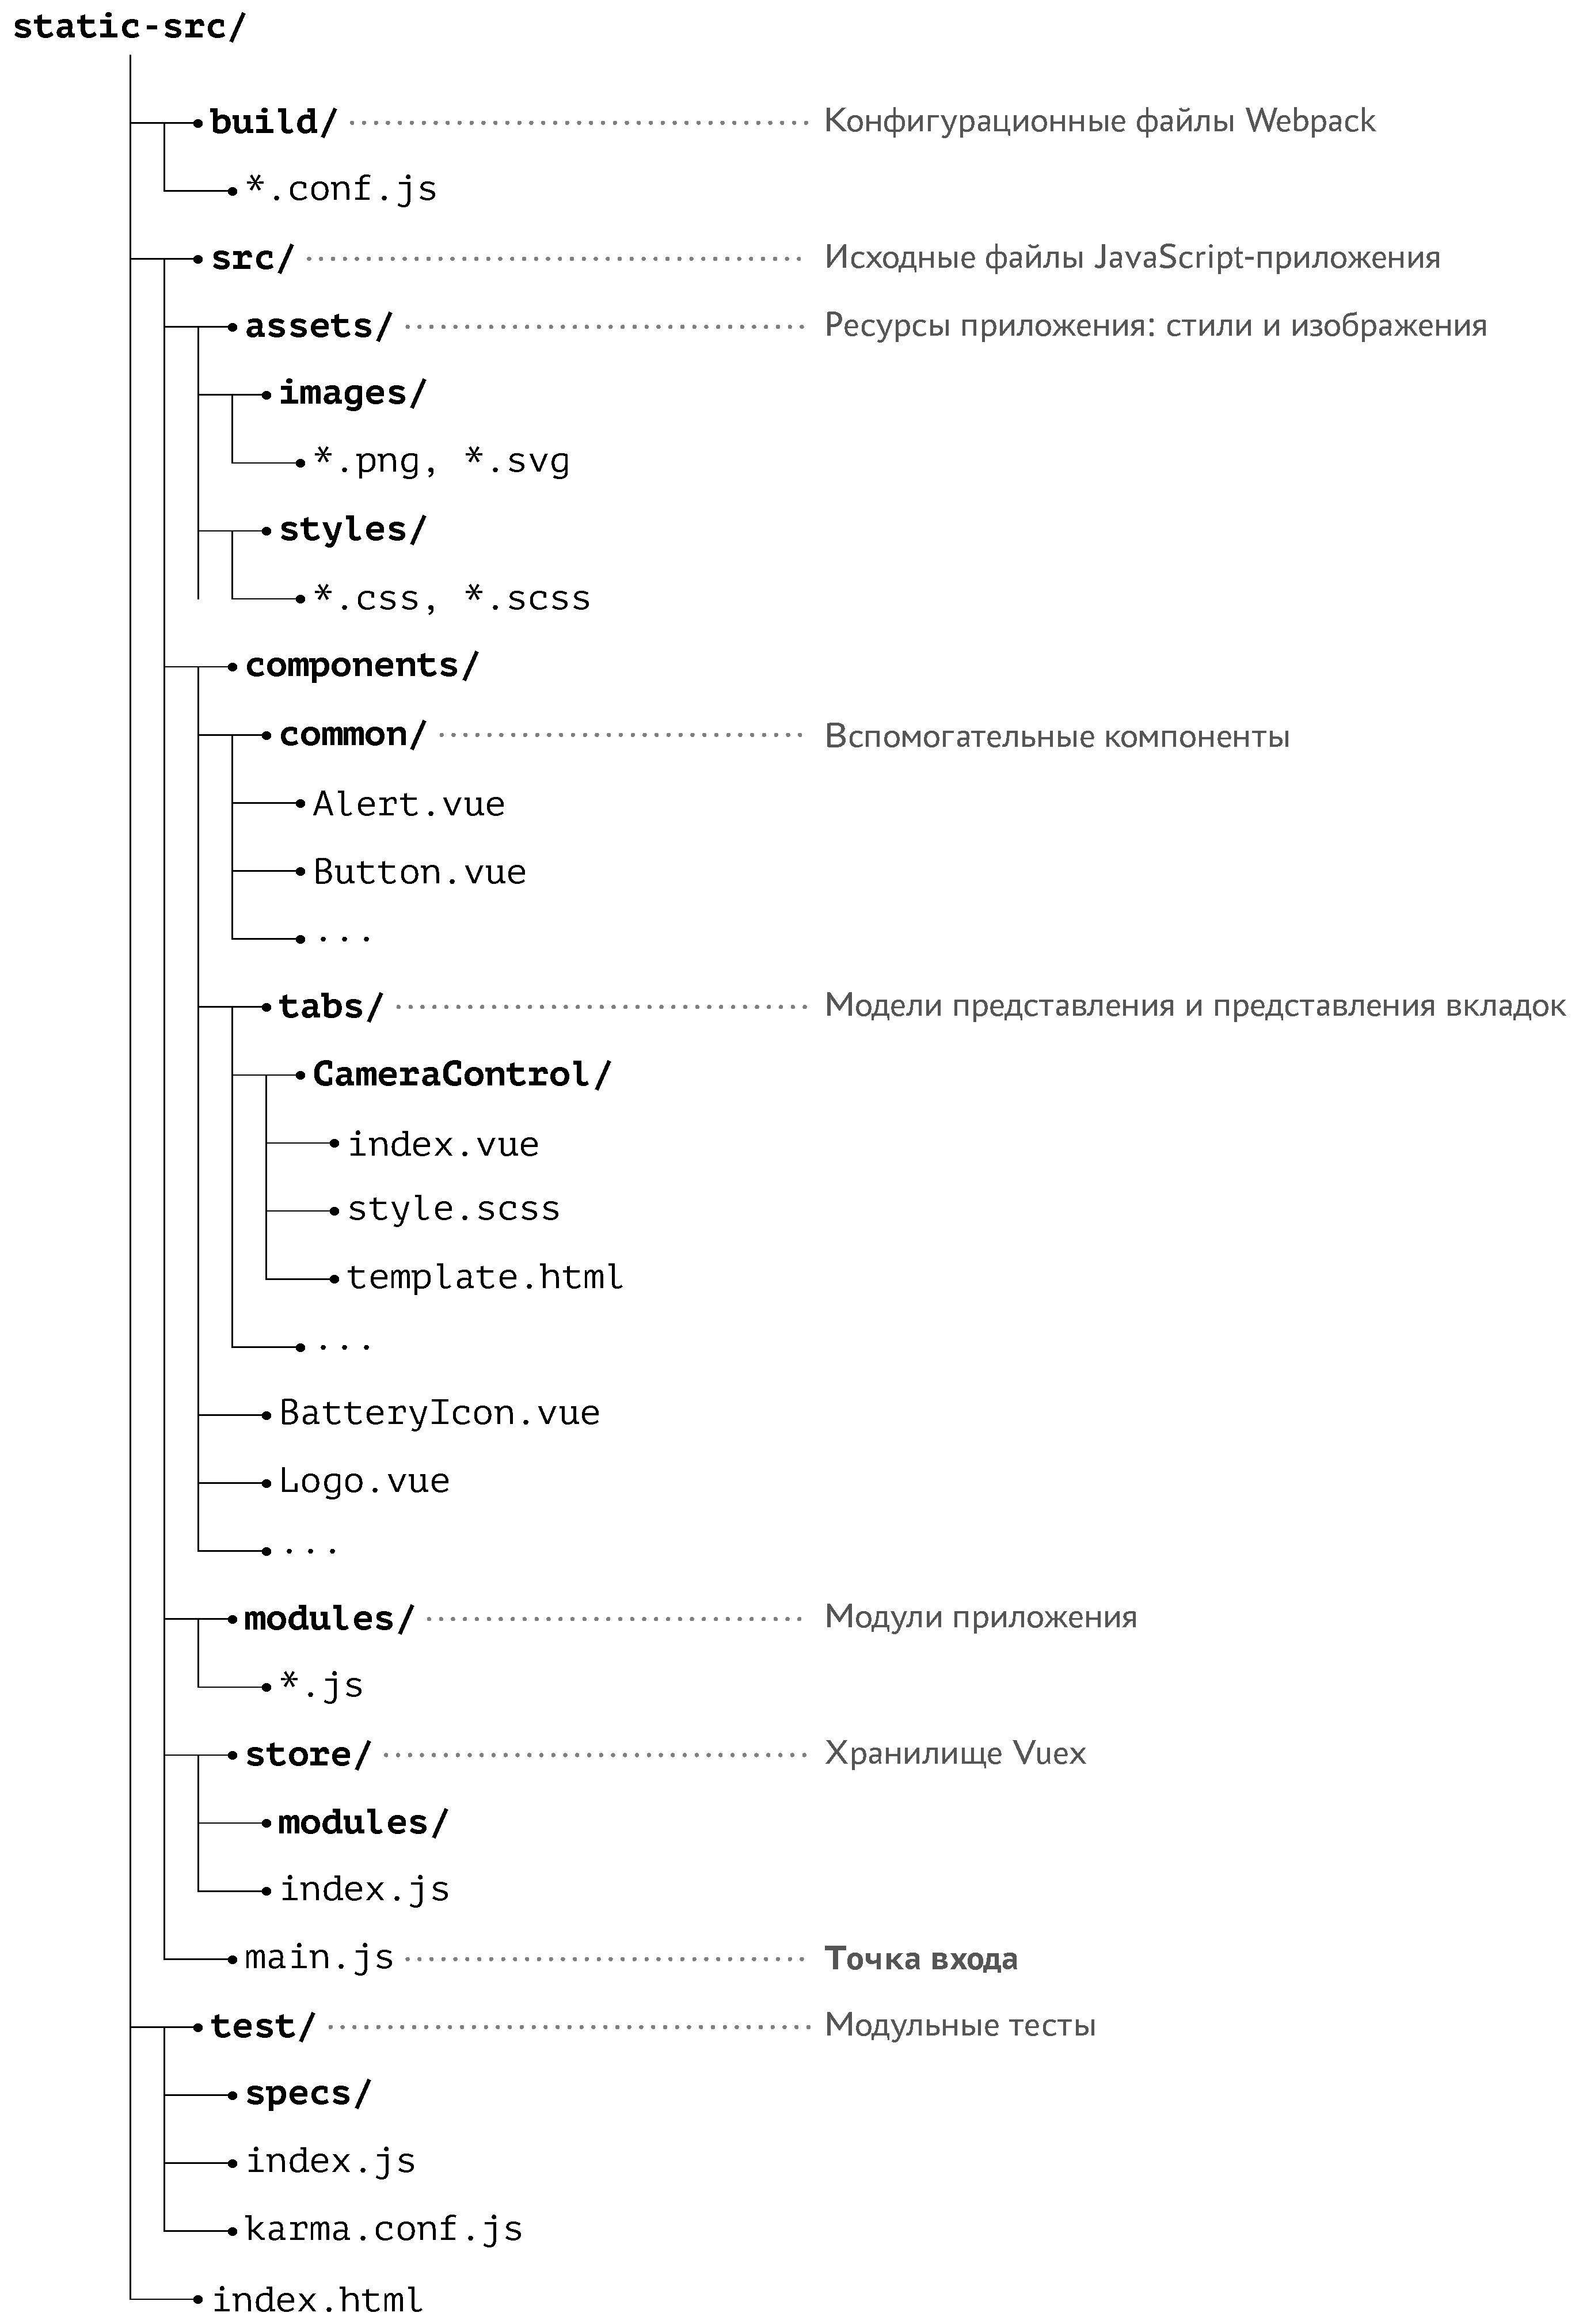
\includegraphics[width=.95\textwidth]{img/tikz/project-tree/pic}
  \vspace*{6pt}
  \caption{Структура проекта}\label{fig:project-tree}
\end{figure}


\subsubsection{Точка входа}


\subsubsection{Артефакты сборки}



\subsection{Глобальное хранилище данных приложения. Однонаправленный поток данных}

\textbf{Vuex} -- библиотека-расширение для Vue.js приложений, позволяющая создавать глобальное хранилище данных, доступное для всех модулей и Vue-компонентов, входящих в~состав проекта. Подобное хранилище необходимо не только для обмена данными между компонентами -- основной его задачей является управление состоянием представлений приложения.

Идеи, лежащие в~основе данной библиотеки, унаследованы от архитектуры Flux \cite{Flux}. Vuex предоставляет шаблонный подход к~управлению состояниями компонентов приложения, основанный на \emph{однонаправленном потоке данных}.


\subsubsection{Однонаправленный поток данных}

Взаимный обмен данными и~событиями между моделями и~представлениями при наличии большого числа компонентов является потенциальным источником ошибок. Асинхронные изменения и~побочные эффекты могут существенно усложнить разработку и~отладку, а~также нарушить работу приложения.

% TODO Добавить "переход" к этому абзацу
Однонаправленный поток данных в~простейшем виде представлен на рисунке \ref{fig:simple-oneway-data-flow}.

\begin{figure}[h!]
  \centering
  \setlength{\fboxsep}{5pt}
  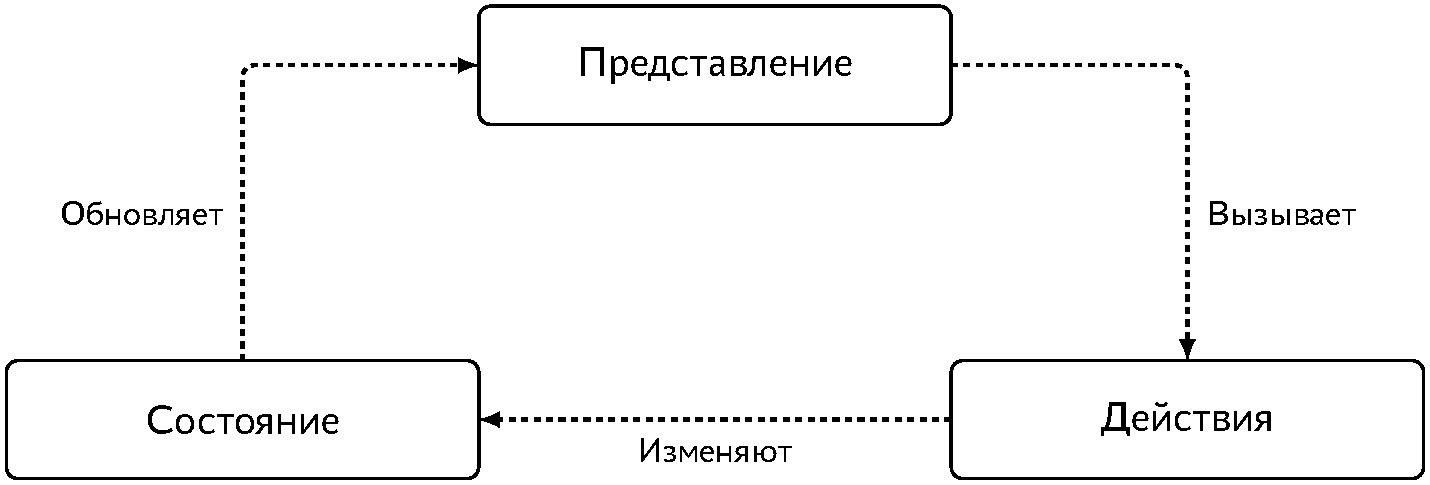
\includegraphics[width=.9\textwidth]{img/tikz/simple-oneway-data-flow/pic}
  \vspace*{12pt}
  \caption{Однонаправленный поток данных}\label{fig:simple-oneway-data-flow}
\end{figure}

Подход, описанный на рисунке \ref{fig:simple-oneway-data-flow}, прекрасно подходит для управления представлением одного компонента. Однако, при появлении нескольких компонентов, зависящих от одного и~того же состояния, структура приложения может существенно усложниться.

% TODO Сноска про <<одиночку>>?
Vuex решает проблему, описанную выше, вводя в~структуру приложения глобальное хранилище данных, являющееся состоянием-<<одиночкой>> (англ. \emph{singleton}), которое обновляет все необходимые представления с~помощью реактивных обновлений.

Для избежания неконтролируемых изменений состояния в~Vuex введено следующее ограничение: изменить состояние можно только с~помощью синхронных транзакций, называемых \emph{мутациями}.

Асинхронные операции, результаты выполнения которых изменяют состояние, в~Vuex получили название \emph{<<действия>>}. Внутри функций-обработ-чиков действий становится возможно, к~примеру, совершить асинхронный запрос к~серверу, а~при получении результата сделать одну или более синхронных мутаций состояния.

Схема организации однонаправленного потока данных при использовании Vuex изображена на рисунке \ref{fig:vuex-oneway-data-flow}.

\begin{figure}[h!]
  \centering
  \setlength{\fboxsep}{5pt}
  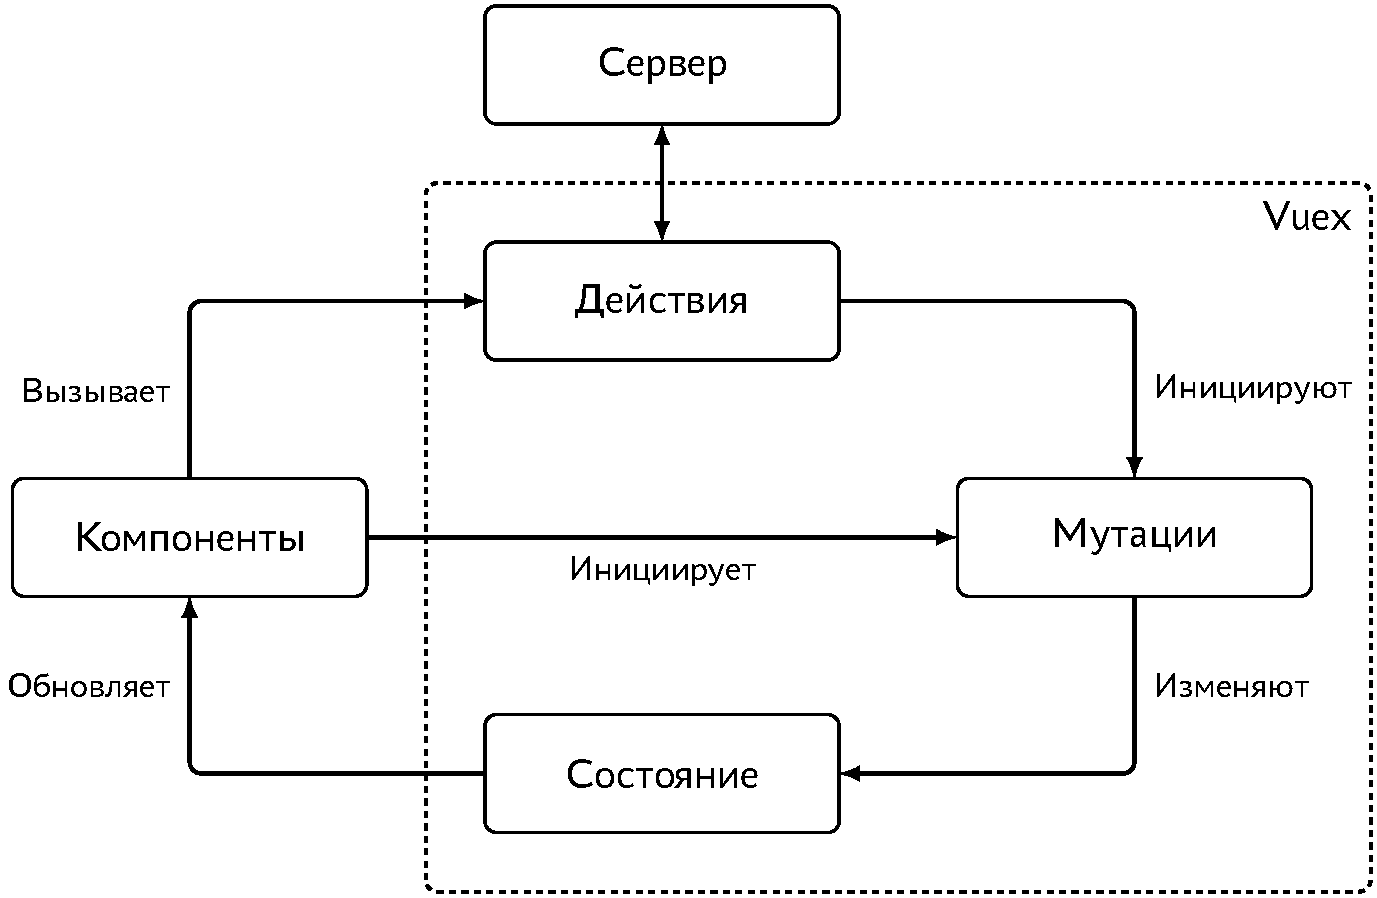
\includegraphics[width=.9\textwidth]{img/tikz/vuex-oneway-data-flow/pic}
  \vspace*{12pt}
  \caption{Однонаправленный поток данных при использовании Vuex}\label{fig:vuex-oneway-data-flow}
\end{figure}


\subsubsection{Модули хранилища данных}

Глобальные данные о~состоянии приложения по умолчанию хранятся в~одном и~том же объекте. Рост числа модулей приложения неизбежно приводит к~тому, что структура данного объекта существенно усложняется, а~именование мутаций и~действий может вызывать затруднения из-за требования к~уникальности имён сущностей Vuex.

Для решения описанных выше проблем Vuex предоставляет инструменты для разделения хранилища на \emph{модули}. Модули представляют из себя самостоятельные части глобального состояния, каждая из которых может содержать объект с~данными, мутации и~т.д. При использовании данного подхода возможные проблемы с~именованием решаются благодаря тому, что каждый модуль Vuex может иметь собственное пространство имён.

% TODO Добавить пример работы с модулями

Хранилище Vuex, используемое в разрабатываемом приложении, было разделено на модули, соответствующие важнейшим подсистемам программного обеспечения устройств Reach и~Reach~RS:
\begin{dashitemize}
  \item информация об устройстве и его конфигурация (модули \emph{device} и \emph{settings});
  \item позиционирование и~режим RTK (модуль \emph{status});
  \item входящие и~исходящие потоки данных (модуль \emph{streams});
  \item беспроводные соединения (модуль \emph{wireless});
  \item изыскания (модуль \emph{survey});
  \item состояние компонентов графического интерфейса (модуль \emph{ui}).
\end{dashitemize}

Схема модулей глобального хранилища изображена на рисунке \ref{fig:vuex-modules}.

\begin{figure}[h!]
  \centering
  \setlength{\fboxsep}{5pt}
  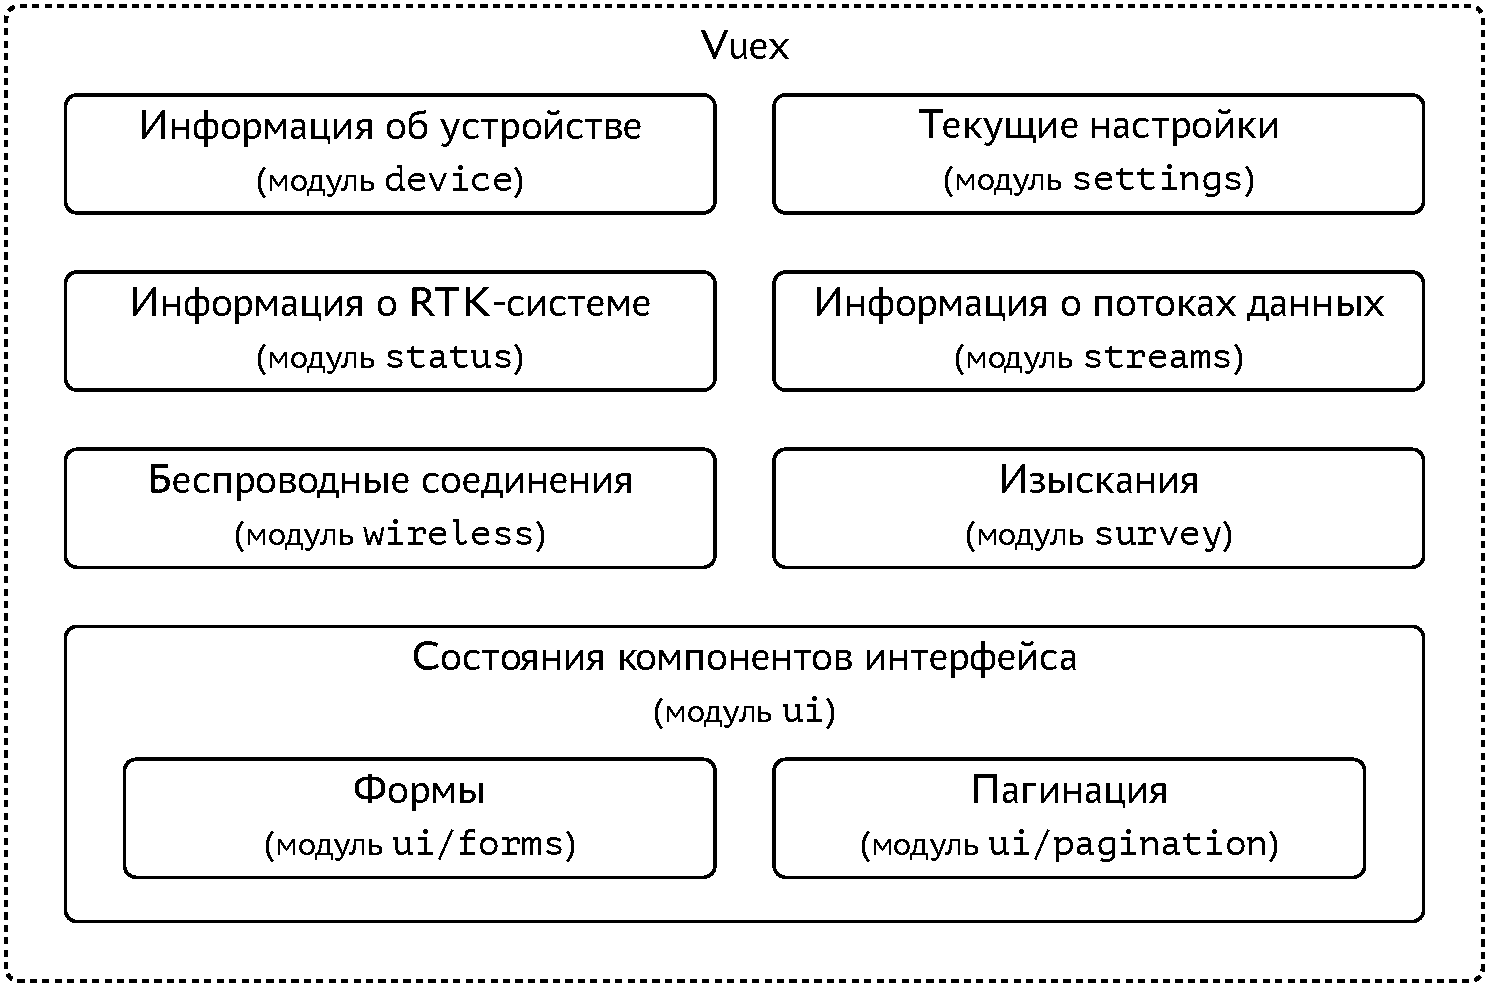
\includegraphics[width=.9\textwidth]{img/tikz/vuex-modules/pic}
  \vspace*{6pt}
  \caption{Модульная структура хранилища Vuex}\label{fig:vuex-modules}
\end{figure}



\subsection{Модули и~компоненты приложения}

В пунктах, следующих далее, описана структура и~организация модулей и~компонентов разрабатываемого веб-приложения. Первые два пункта посвящены модулям общего назначения и~вспомогательным компонентам, которые необходимы для создания моделей представления, описанных в~подразделе \ref{subsec:app-modules-requirements}. Сами же модели представления описаны в~третьем пункте текущего подраздела.


\subsubsection{Модули общего назначения}

К~модулям общего назначения относятся модуль работы с~картами и~модуль обработки событий. Рассмотрим каждый из их подробнее.

\paragraph{Модуль работы с~картами}

Модуль работы с~картами представляет из себя обёртку (англ. \emph{wrapper}) над частью библиотеки OpenLayers, используемой в~разрабатываемом приложении для отображения карт и различной информации на них. Код модуля содержится в~файле \emph{olWrapper.js}.

Данный модуль предназначен для повышения удобства создания однотипных карт -- для добавления карты на определённую страницу достаточно импортировать модуль в нужную часть кода приложения и~вызвать соответствующие функции.

Импорт необходимых модулей OpenLayers, единожды осуществляемый в~модуле работы с~картами (см.~листинг \ref{lst:modules__maps__imports}), исключает повторение существенного количества строк кода и~уменьшает размер файла vendor.js.

\lstinputlisting[
  caption={olWrapper.js: импорт необходимых модулей OpenLayers},
  label={lst:modules__maps__imports}
]{src/modules__maps__imports.js}

% TODO Добавить полный листинг в Приложения


\paragraph{Модуль обработки событий}

Модуль обработки событий (\emph{eventsModule.js}) выполняет ряд ключевых задач, необходимых для работы приложения:
\begin{dashitemize}
  \item инициализация WebSocket-подключения;
  \item обработка разрыва (восстановления) соединения с сервером;
  \item оповещение пользователя о различных событиях.
  \item инициализация модулей Vuex путём вызова их действий.
\end{dashitemize}

В листинге \ref{lst:modules__events__short} представлено содержимое файла eventsModule.js (полный листинг файла см. в приложении ??). По умолчанию модуль экспортирует функцию, выполнение которой зарегистрирует несколько слушателей событий Socket.IO и вызовет действие \emph{<<activate>>} (\emph{activate} с англ. -- <<активировать>>) в четырёх модулях Vuex.

Действия с названием <<activate>> присутствуют во всех модулях Vuex, кроме модулей, отвечающих за хранение состояния компонентов интерфейса (см. рис.~\ref{fig:vuex-modules}). <<Активация>> модуля Vuex подразумевает под собой:
\begin{dashitemize}
  \item установка значений по умолчанию в объекте состояния (при необходимости);
  \item регистрация слушателей определённых широковещательных сообщений сервера;
  \item отправка на сервер запросов на получение данных;
  \item создание таймеров для периодических опросов сервера.
\end{dashitemize}

\lstinputlisting[
  caption={Модуль обработки событий},
  label={lst:modules__events__short}
]{src/modules__events__short.js}

Также модуль обработки событий экспортирует объект \emph{socket}, импортируя который, любой компонент приложения сможет осуществлять общение с сервером через WebSocket-события.


\subsubsection{Вспомогательные компоненты}

Вспомогательные компоненты представляют из себя набор блоков и элементов интерфейса, необходимых для создания всевозможных представлений приложения. Данные компоненты включают в себя кнопки, переключатели, панели, индикаторы выполнения и т.д. (см. рис.~\ref{fig:common-components}). На рисунке \ref{fig:form-example} представлен пример формы, составленной из вспомогательных компонентов.

\begin{figure}[h!]
  \centering
  \setlength{\fboxsep}{5pt}
  \subfloat[\label{sub:common-components__buttons}]{
    \includegraphics[width=.25\textwidth]{example-image-a}
  }
  \qquad
  \subfloat[\label{sub:common-components__toggles}]{
    \includegraphics[width=.25\textwidth]{example-image-b}
  }
  \vspace*{6pt}
  \caption{
    Пример вспомогательных компонентов:\\
    \protect\subref{sub:common-components__buttons} - кнопки,
    \protect\subref{sub:common-components__toggles} - переключатели
  }
  \label{fig:common-components}
\end{figure}

\begin{figure}[h!]
  \centering
  \setlength{\fboxsep}{5pt}
  \includegraphics[width=.75\textwidth]{example-image}
  \vspace*{6pt}
  \caption{Пример формы, составленной из вспомогательных компонентов}
  \label{fig:form-example}
\end{figure}

Каждый вспомогательный элемент является Vue-компонентом, что даёт возможность управлять внешним видом, содержимым и поведением каждого из них. К примеру, компонент <<переключатель>> (англ. \emph{toggle}) кроме обязательного параметра, являющегося булевой переменной, также позволяет настроить свой текст, цвет и доступность для изменения состояния (см. листинг~\ref{lst:component__common__toggle__short}).

\newpage

\lstinputlisting[
  caption={Настраиваемые свойства компонента <<переключатель>>},
  label={lst:component__common__toggle__short}
]{src/component__common__toggle__short.vue}


\subsubsection{Модели представления и представления}

\paragraph{Статус}

<<Статус>> является представлением, отображаемым по умолчанию. Основная задача данного представления -- вывод информации об RTK-системе, сигналах спутников и позиции приёмника.

<<Статус>> зависит от данных, содержащихся в модуле status хранилища Vuex. Модуль status содержит всю необходимую для вывода информацию, обновляемую в режиме реального времени благодаря реактивности Vuex и зарегистрированным слушателям широковещательных сообщений сервера.

На рисунке \ref{fig:status-detailed} изображена страница <<Статус>>, отображающая состояние ровера, получающего поправки с базы. Набор элементов страницы и их отображение меняется, в зависимости от наличия (отсутствия) тех или иных данных, а также от режима работы RTKLIB. Так, например, столбчатая диаграмма значений соотношений сигнал/шум для принимаемых со спутников сигналов примет вид, изображённый на рисунке \ref{fig:status-snr-rover}, при отсутствии данных о спутниках, видимых базе. Другим примером может служить скрытие элементов ?? и ?? при переводе RTKLIB в режим Single (см. пункт \ref{subsec:rtklib-modes}).

% TODO Сделать нормальную картинки
\begin{figure}[h!]
  \centering
  \setlength{\fboxsep}{5pt}
  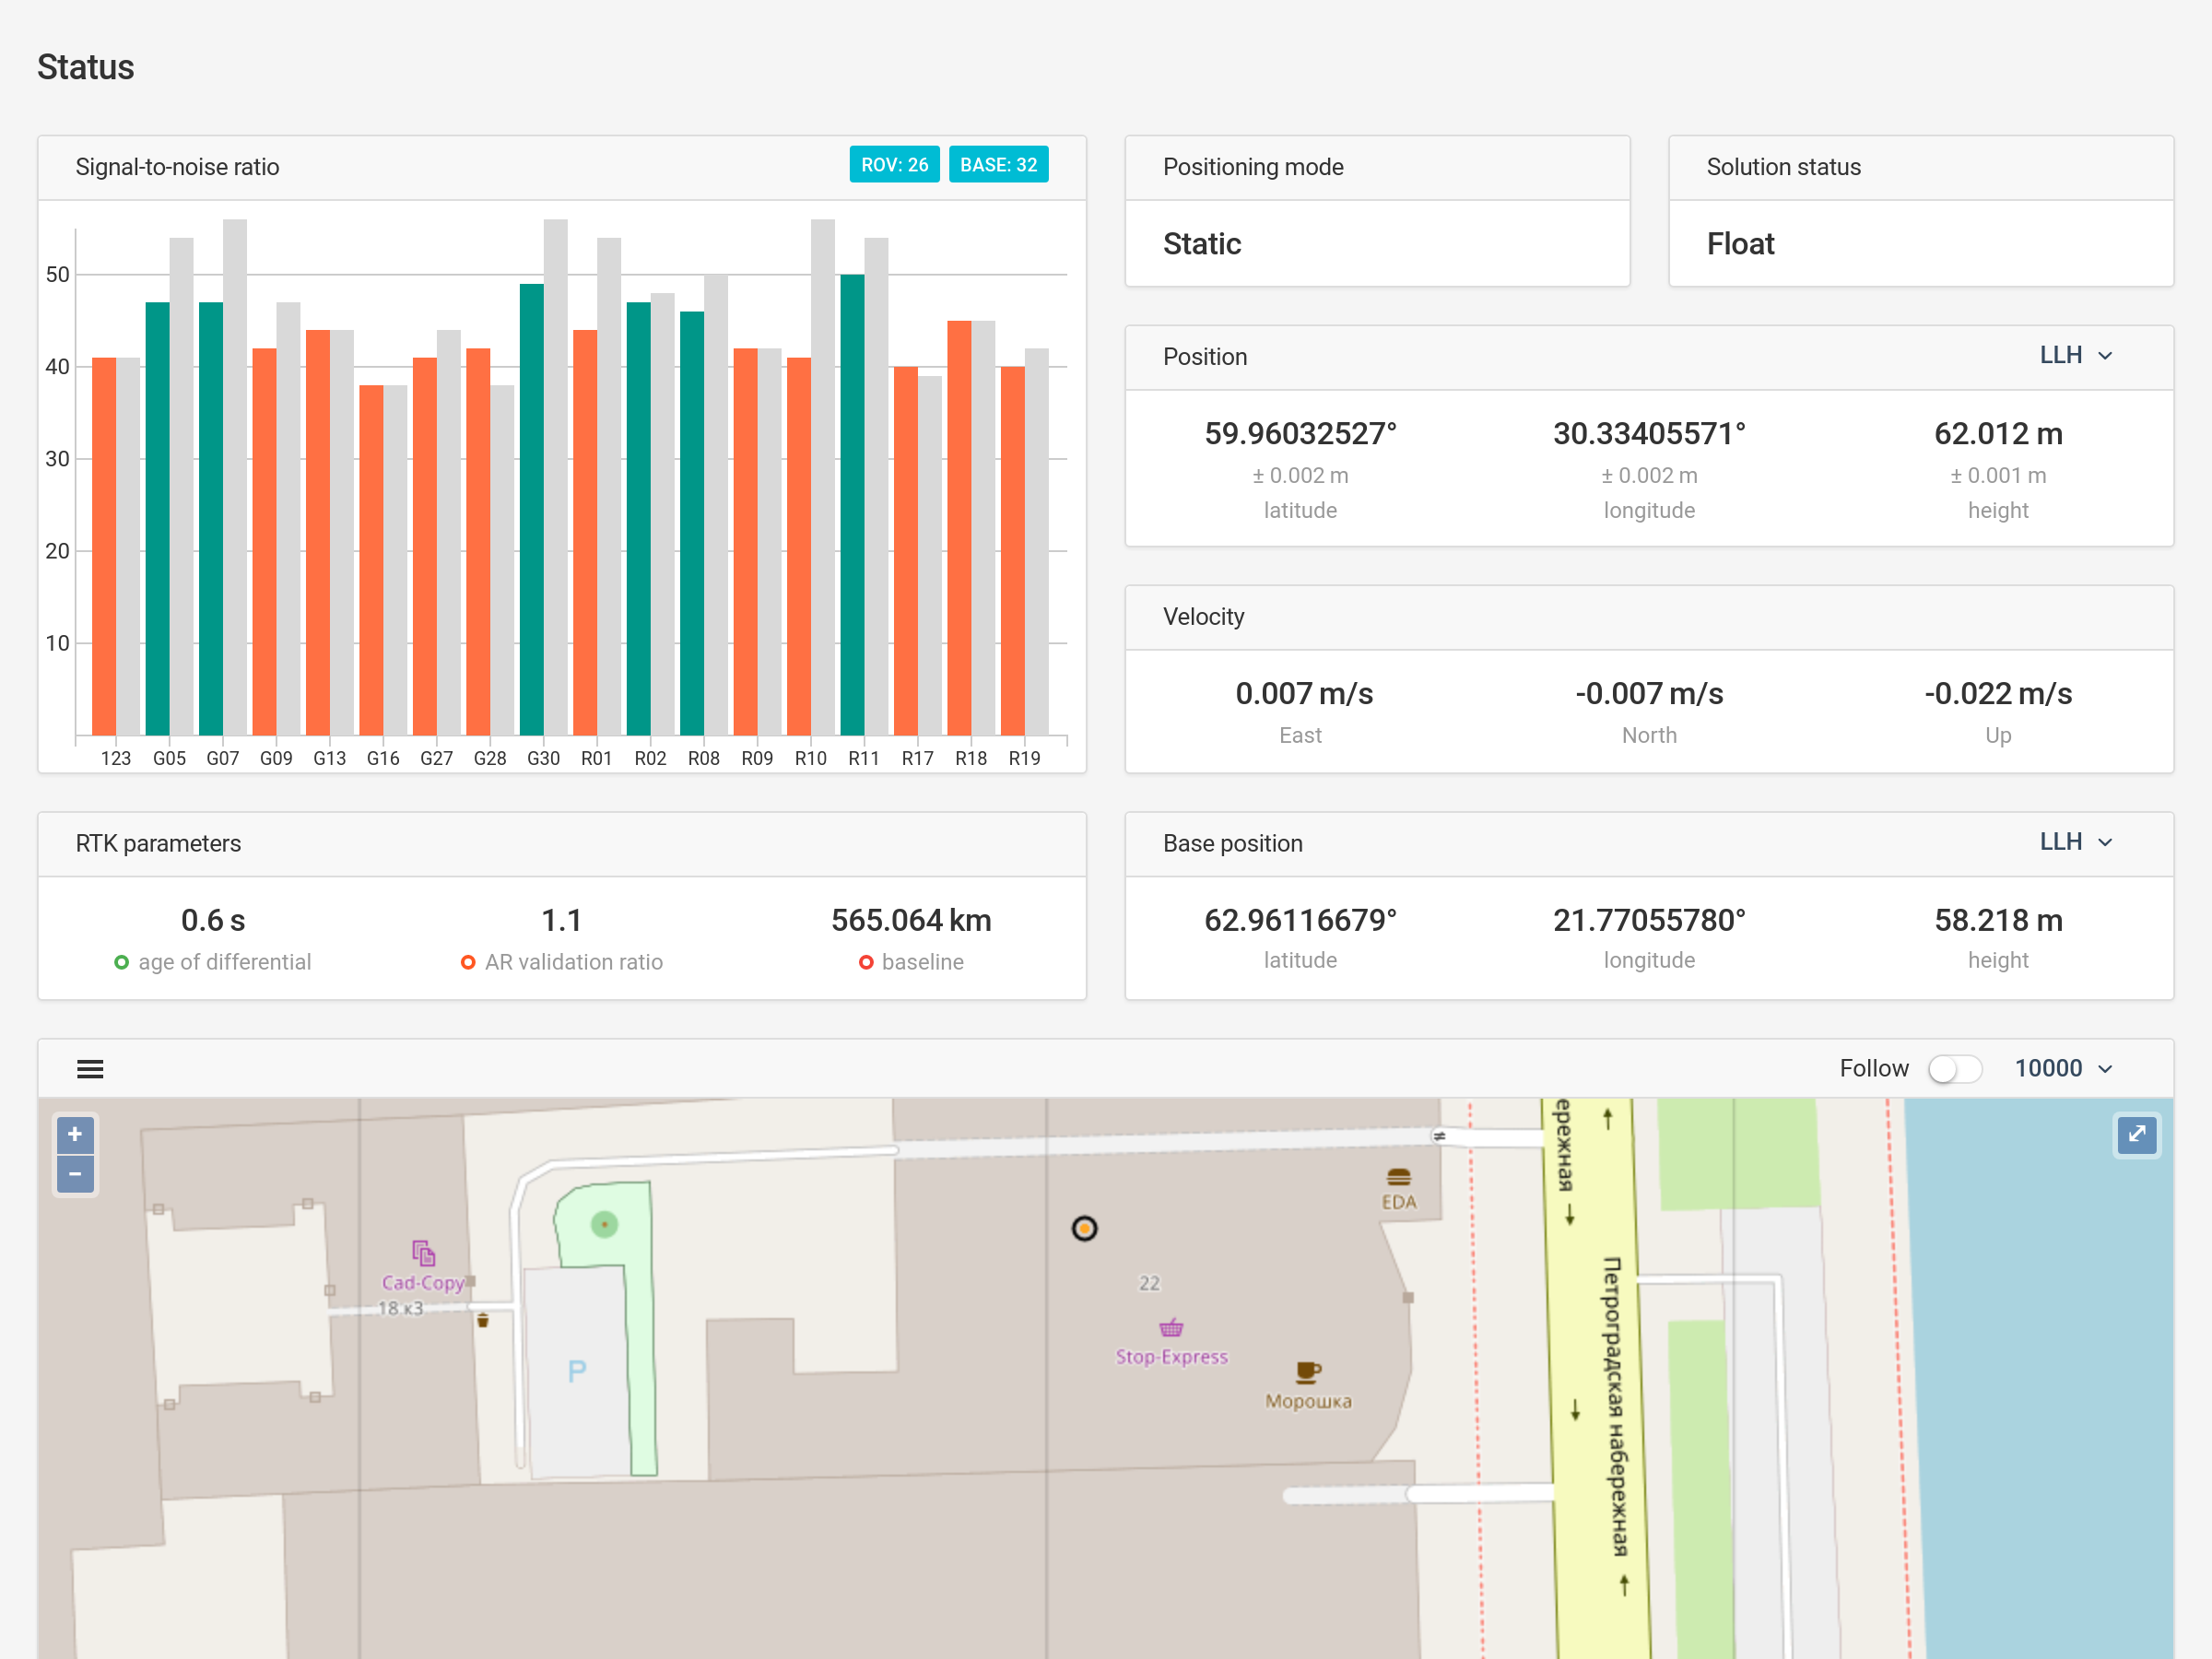
\includegraphics[width=.9\textwidth]{img/reachview/status_content_laptop}
  \vspace*{6pt}
  \caption{Страница <<Статус>>}
  \label{fig:status-detailed}
\end{figure}

\begin{figure}[h!]
  \centering
  \setlength{\fboxsep}{5pt}
  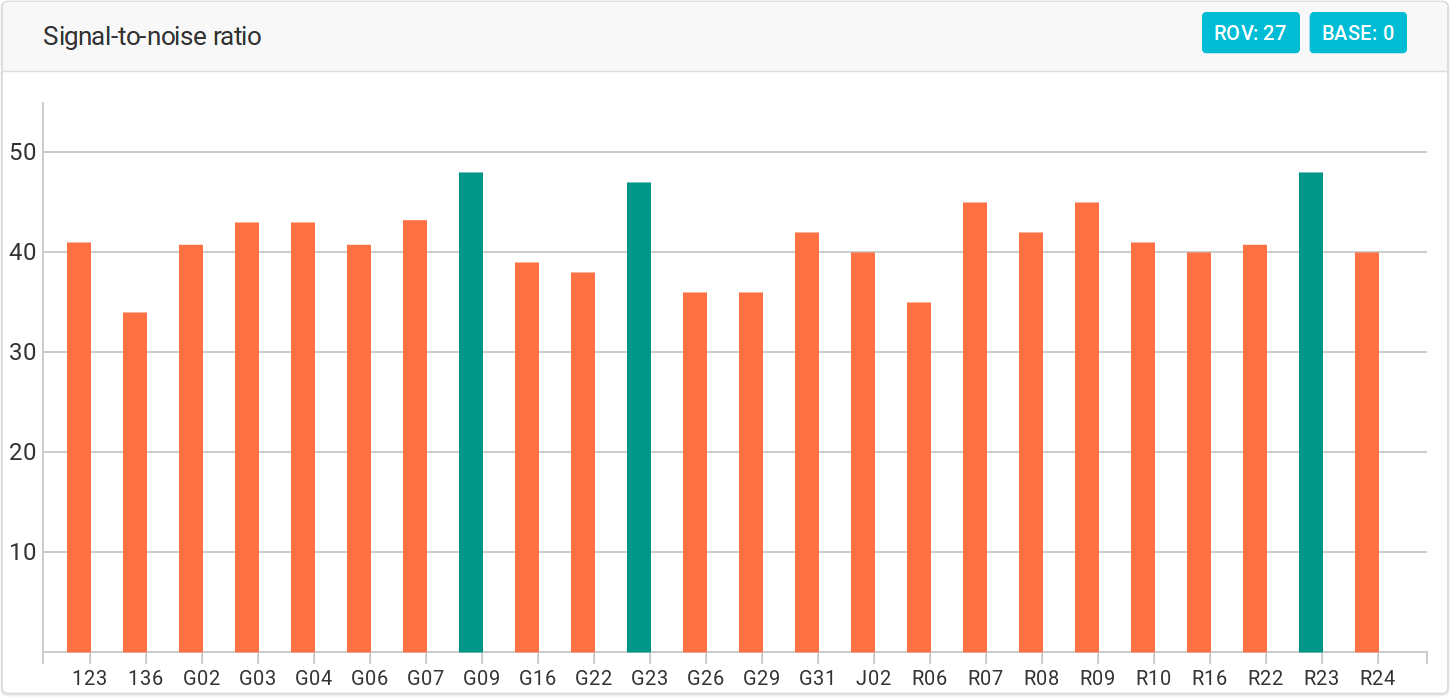
\includegraphics[width=.9\textwidth]{img/reachview/status_snr_rover}
  \vspace*{6pt}
  \caption{Отсутствие данных о спутниках, видимых базе}
  \label{fig:status-snr-rover}
\end{figure}

\paragraph{Изыскания}

<<Изыскания>> -- раздел приложения, с помощью которого происходит основная часть работы с устройством. Используя данный интерфейс пользователь может производить геодезические изыскания -- сбор точек на местности, с разделением их на проекты.

В соответствии с требованиями, перечисленными в пункте \ref{subsec:survey-requirements}, был разработан модуль приложения, основанный на сущностях и прецедентах, описанных на рисунках \ref{fig:survey-uml-classes} и \ref{fig:survey-uml-usecase} соответственно.

\begin{figure}[h!]
  \centering
  \setlength{\fboxsep}{5pt}
  \includegraphics[width=.75\textwidth]{example-image}
  \vspace*{6pt}
  \caption{Диаграмма классов модуля <<Изыскания>>}
  \label{fig:survey-uml-classes}
\end{figure}

\begin{figure}[h!]
  \centering
  \setlength{\fboxsep}{5pt}
  \includegraphics[width=.75\textwidth]{example-image}
  \vspace*{6pt}
  \caption{Диаграмма прецедентов модуля <<Изыскания>>}
  \label{fig:survey-uml-usecase}
\end{figure}

Модуль <<Изыскания>> состоит из множества отдельных представлений, переключаясь между которыми, пользователь осуществляет разнообразные действия с собранными данными. Одной из основных задач при разработке данного модуля было чёткое описание возможных состояний и условий перехода между ними. На рисунке \ref{fig:survey-uml-state} представлена диаграмма состояний модуля <<Изыскания>>.

\begin{figure}[h!]
  \centering
  \setlength{\fboxsep}{5pt}
  \includegraphics[width=.75\textwidth]{example-image}
  \vspace*{6pt}
  \caption{Диаграмма состояний модуля <<Изыскания>>}
  \label{fig:survey-uml-state}
\end{figure}

\paragraph{Модули настройки параметров работы устройства}

\paragraph{Модули настройки входящих и исходящих потоков данных}

\paragraph{Модули настройки беспроводных соединений}

\paragraph{Общие настройки}

\newpage
